\chapter{Stål}
INDLEDNING

\section{Reaktionskræfter}
Reaktionskræfterne til det statiske system skal bestemmes. Der er opstillet en indvendig stålkonstruktion, se Figur \ref{fig:system}, til optagelse af lasterne på bygning. Som det ses på figuren, indeholder konstruktion tre rammer, der er opsat. På rammerne vil lasterne fra taget og etagedækkene optages. Taget i bjælkekonstruktionen er forbundet til den resterende del af konstruktionen via charnierledene. Belastningerne der virker på taget vil dermed kunne overføres til den resterende del af konstruktionen som funktlaster med angrebspunkt i kundepunkterne hvor charnierledene er, som kan ses på Figur \ref{fig:del2}. 

\begin{figure}[htbp]
	\centering
	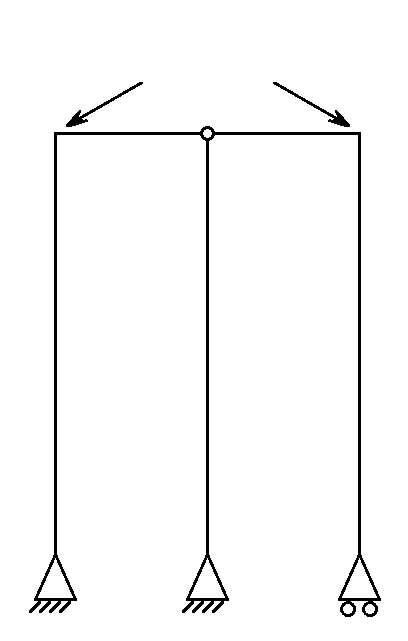
\includegraphics[width=0.3\textwidth]{billeder/delto.png}
	\caption{Laster fra taget optages i charnierledene}
	\label{fig:del2}
\end{figure}

Når der beregnes reaktionskræfter for de tre understøtninger, er der behov for at opdele konstruktionen. Systemet opdeles i det midterste charnierled i henholdvis en højre- og venstre del, som ses på Figur \ref{fig:opdeling}. I skæringen mellem de to dele, vil der være snitkræfter men ikke momentkræfter, da momentet i charnierledet er nul. Dermed optræder der kun normalkraft, N, og forskydningskraften, V.

\begin{figure}[htbp]
	\centering
	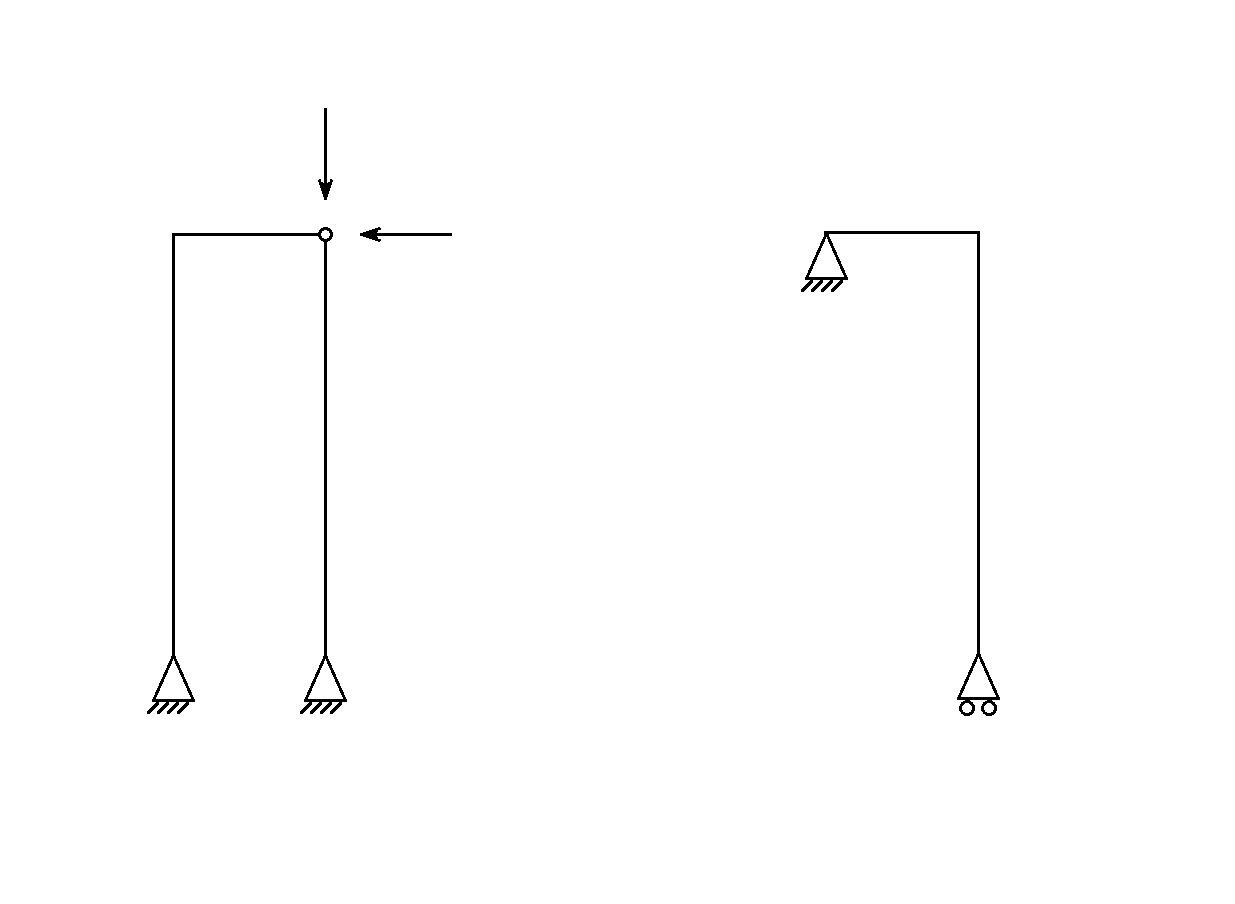
\includegraphics[width=0.5\textwidth]{billeder/systemopdeling.png}
	\caption{Opdeling af det statiske system}
	\label{fig:opdeling}
\end{figure}
 
\section{Snitkræfter}
Både snitkræfter og snitkræftskurver.

\section{Spænding}
Spændingsfordeling af normalspænding og forskydningsspænding.

\section{...}
Brudgrænsetilstand, nedbøjning mm?...